\documentclass[]{standalone}
\usepackage{tikz}
\usetikzlibrary{shapes,arrows,calc,positioning}
\usepackage{amsmath} % for dfrac
\usepackage{comment}
\usepackage{calc}

% definition of basic block
\tikzset{
    block/.style = {draw, rectangle,
        minimum height=1.2cm,
        minimum width=2cm},
    input/.style = {coordinate,node distance=1cm},
    output/.style = {coordinate,node distance=1cm},
    sum/.style = {draw, circle, node distance=1cm},
}

% definition of saturation block
\tikzset{% from https://tex.stackexchange.com/questions/161075/saturation-block
  saturation block/.style={%
    draw, 
    path picture={
      % Get the width and height of the path picture node
      \pgfpointdiff{\pgfpointanchor{path picture bounding box}{north east}}%
        {\pgfpointanchor{path picture bounding box}{south west}}
      \pgfgetlastxy\x\y
      % Scale the x and y vectors so that the range
      % -1 to 1 is slightly shorter than the size of the node
      \tikzset{x=\x*.4, y=\y*.4}
      %
      % Draw annotation
      \draw (-1,0) -- (1,0) (0,-1) -- (0,1); 
      \draw (-1,-.7) -- (-.6,-.7) -- (.6,.7) -- (1,.7);
    }
  }
}
\tikzset{% from https://tex.stackexchange.com/questions/161075/saturation-block
  deadband block/.style={%
    draw, 
    path picture={
      % Get the width and height of the path picture node
      \pgfpointdiff{\pgfpointanchor{path picture bounding box}{north east}}%
        {\pgfpointanchor{path picture bounding box}{south west}}
      \pgfgetlastxy\x\y
      % Scale the x and y vectors so that the range
      % -1 to 1 is slightly shorter than the size of the node
      \tikzset{x=\x*.4, y=\y*.4}
      %
      % Draw annotation
      \draw (-1,0) -- (1,0) (0,-1) -- (0,1);  % axis
      \draw (-1,1) -- (-.3,.3) -- (-.3,0) -- (.3,0) -- (.3,-.3) -- (1,-1);
	  %\draw (-.3,.3) -- (.3,-.3) ;
    }
  }
}

\begin{document}
	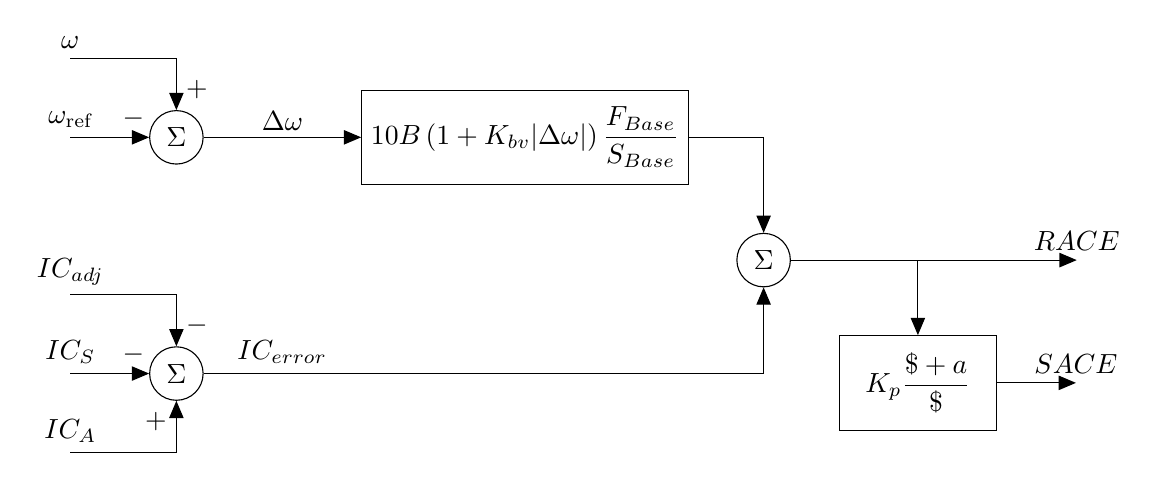
\begin{tikzpicture}[auto, node distance=1cm,>=triangle 45]
		% Starting inputwref
		\node [input, name=inputwref, label=$\omega_{\text{ref}}$]  {};
		% Starting inputw
		\node [input, name=inputw, above=of inputwref, label=$\omega$] (inputw) {};
		% sum 1
		\node [sum, right=of inputwref] (sum1) {$\Sigma$};
		% delta w node and label
		\coordinate [right=of sum1]  (deltaw) {};
		\coordinate [above=-.1em of deltaw,label={$\Delta\omega$}]  (deltaWlabel){};
		
		
		% input ICsched
		\node [input, name=ICsched, below=3 cm of inputwref, label=$IC_{S}$] {};
		% input IC
		\node [input, name=IC, below=of ICsched, label=$IC_A$] {};
		% input ICadjust
		\node [input, name=ICadj, above=of ICsched, label=$IC_{adj}$] {};
		% sum 2
		\node [sum, right=of ICsched] (sum2) {$\Sigma$};
		
		% Frequnecy Bias block
		\node [block, right=of deltaw] (fbias) {$10B \left(1+K_{bv} |\Delta \omega| \right) \dfrac{F_{Base}}{S_{Base}}$};
		
		% RACE summing
		\node [sum, below right=1cm of fbias] (RACEsum) {$\Sigma$};		
		
		% Filtering
		\node [block, below right=1cm of RACEsum,] (filter) {$K_p\dfrac{\$ + a}{\$}$};
		
		% output
		\node [output, right=of filter, label=$SACE$] (output) {};		
		\node [output, right=3.63cm of RACEsum, label=$RACE$] (output2) {};
		
		% connecting lines
		\draw [draw,->] (inputwref) -- node[pos=0.8] {$-$} (sum1); 
		\draw [->] (inputw) -| node[pos=0.8] {$+$} (sum1);
		\draw [->] (sum1) -- (fbias);
		\draw [draw,->] (ICsched) -- node[pos=0.8] {$-$} (sum2); 
		
		\draw [draw,->] (ICadj) -| node[pos=0.8] {$-$} (sum2); 
		
		\draw [->] (IC) -| node[pos=0.8] {$+$} (sum2);
		\draw [->] (fbias) -| (RACEsum);
		\draw [->] (sum2) -| node[pos=0.07] {$IC_{error}$}(RACEsum); 		
		
		\draw [->] (RACEsum) -| (filter);
		\draw [->] (filter) -- (output);
		\draw [->] (RACEsum) -- (output2);
	\end{tikzpicture} 
\end{document}